%% LyX 2.3.3 created this file.  For more info, see http://www.lyx.org/.
%% Do not edit unless you really know what you are doing.
\documentclass[french, twocolumn]{article}
\usepackage[T1]{fontenc}
% \usepackage[latin9]{inputenc}
\RequirePackage[utf8]{inputenc}
\usepackage[a4paper]{geometry}
\geometry{verbose,tmargin=2cm,bmargin=2cm,lmargin=2cm,rmargin=2cm}
\setlength{\parindent}{0bp}
\usepackage[french]{babel}
\usepackage{textcomp}
\usepackage{amsmath}
\usepackage{float}
\usepackage{biblatex}[
    backend=biber,        % compilateur par défaut pour biblatex
    sorting=nyt,          % trier par nom, année, titre
    citestyle=authoryear, % style de citation auteur-année
    bibstyle=alphabetic,  % style de bibliographie alphabétique
]
\usepackage[unicode=true]
 {hyperref}
\addbibresource{biblio.bib}
\usepackage{fancyhdr}
\usepackage{comment}
\usepackage{caption}
\usepackage{subcaption}
\usepackage{graphicx}

\makeatletter
%%%%%%%%%%%%%%%%%%%%%%%%%%%%%% Textclass specific LaTeX commands.
\newcommand{\lyxaddress}[1]{
	\par {\raggedright #1
	\vspace{1.4em}
	\noindent\par}
}

\@ifundefined{date}{}{\date{}}
\makeatother

\begin{document}
\title{Instruction for authors - Latex template}
\author{
C. Fernandez, P. Jardin, V. Piton, H. Audas, P. Estève, B. Quiédeville}
\maketitle



% \lyxaddress{$^{3}$ CNRS, UPR 7051, Aix-Marseille Univ, Centrale Marseille, F-13453
% Marseille Cedex 13, France }

% \lyxaddress{$^{*}$ Corresponding author, scotti@lma.cnrs-mrs.fr}
\begin{abstract}
    Ceci est notre abstract
\end{abstract}

% Default content with instructions
% \begin{abstract}
Instead of providing a classic template to be filled in by the authors,
we decided to present an example on how to build \textbackslash LaTeX\{\}
source files to be published in Acta Acustica. 

Authors are free to follow any style for the article and references,
as long as it is internally consistent. Please consult the \href{https://acta-acustica.edpsciences.org/author-information/instructions-for-authors}{Instructions for Authors}
for more information.
\end{abstract}

\section{General}

\subsection{Aims and scope }

Acta Acustica, the Journal of the \href{https://euracoustics.org/}{European Acoustics Association (EAA)},
is an international, peer-reviewed journal on acoustics. \\

Acta Acustica reports on original scientific research in acoustics
and on engineering applications.\\

The journal considers Review Articles, Scientific Articles, Audio
Articles, Technical and Applied Articles, Short Communications, Letters
to the Editor. Articles can cover all subjects in the field of acoustics,
including:


\section{Manuscripts}

\subsection{Style }

\subsubsection{Formatting text }

Any submitted manuscript should be in a form that allows the referees
efficient study. No special formatting is required, but it should
be:

easily readable; 
\begin{itemize}
\item pages should be consecutively numbered; 
\item on each page lines should be numbered; 
\item Formulae should be clearly written using standard symbols which are
explained at their first appearance. 
\end{itemize}
Nomenclatures or lists of symbols will be dropped.

\subsubsection{Figures}

\subsubsection*{Figure numbers and legends }

Figures should be numbered as Figure 1, Figure 2, etc. They are referred
to in the text as Figure 1, Figure 2, etc. Legends are grouped on
a separate page.

\subsubsection*{Technical information }

All figures are published free of charge (i.e. they are included in
the publication fee), including color photographs and diagrams. However,
only photographs of scientific interest and pertaining to the subject
of the article should be included. Color illustrations, especially
diagrams, should be understandable even, if they are printed as grey
levels.\\

Figures should be prepared to be of good quality both when they are
viewed onscreen as HTML and when the PDF is printed. Figures may be
arranged as \textquotedbl plates\textquotedbl , but keep in mind
that PDFs are prepared to be printed on A4 pages.

The electronic submission system will accept PNG (preferred), TIFF
(with compression), and EPS files, with appropriate resolution (300
dpi for colour photographs, 600 dpi for halftone work, 1200 dpi for
line work). JPG format is not recommended - PNG is preferred.\\

Manuscripts with figures of insufficient technical quality will be
immediately sent back for revision by the editorial team and will
not begin the review process before correct files are uploaded. In
other words, sending a manuscript with incorrect figures will gain
nothing and may delay its possible publication.

\subsection{Bibliography }

Articles submitted to Acta Acustica should cite all relevant work,
part of which should have appeared in Acoustics journals such as Acta
Acustica. This criterion will be applied to determine whether the
article is within scope of the journal.\\

The number of citations should not exceed 80 except for review papers.
References are cited by numbers in rectangular brackets, for example
\cite{key-1,key-2}. The reference list is placed at the end of the
manuscript. The order of references is according to their appearance
in the article. All author names should be included in the reference
(cf. References below).\\

The references shall be presented as the following examples in the
reference list:
\begin{itemize}
\item Journal article: F. Wendling, F. Bartolomei, J.-J. Bellanger, P. Chauvel:
Interpretation of interdependencies in epileptic signals using a macroscopic
physiological model of eeg. Clinical neurophysiology 112 (2001) 1201--1218. 
\item Book: I. Goodfellow, Y. Bengio, A. Courville: Deep Learning. MIT Press,
2016 
\item Book chapter: A. Amendola, D.E. Bonasia: The menisci: Anatomy, healing
response, and biomechanics, in The Knee Joint Bonnin M, Amendola NA,
Bellemans J, MacDonald SJ, Menetrey J, Editors Paris, Heidelberg,
Springer. 2011 
\end{itemize}

\cite{gibiat_phase_1988}
For Latex contributions, if the bibliography is done in an external
.bib file, authors are asked to upload both the .bib and the .bbl
files obtained by a \textquotedblright bibtex\textquotedblleft{} compilation
of the main .tex file on their own computer.\\

The official abbreviation for Acta Acustica is: \textquotedblright Acta
Acust\textquotedblleft .

\subsection{Data Policy }

\subsubsection{FAIR data principles }

Acta Acustica supports the FAIR data principles: data relevant to
research published in an Acta Acustica article should be findable,
accessible, interoperable, and re-usable (see \href{https://www.force11.org/group/fairgroup/fairprinciples}{https://www.force11.org/group/fairgroup/fairprinciples}).\\

The dataset should be findable through a complete set of metadata,
including a license for re-use and a data identifier (DOI or other).
The dataset is accessible when access is open. Interoperable means
that the data can be used and combined with other datasets in a format
that is sufficiently widely distributed. Re-usability is achieved
when the dataset is deposited with a corresponding Creative Commons
open license and is downloadable. Further, re-usability includes that
parameters how this dataset has been collected and machine and experimental
conditions are documented.

\subsubsection{Use of data repositories }

Acta Acustica authors are invited to upload supplemental datasets
related to their research to an appropriate public data repository,
under a Creative Commons (CC) licence. This makes the data available
for both human and machine reading in order to further aid the acceleration
of scientific discovery. Data repositories generate a unique and persistent
data identifier such as a digital object identifier (DOI), making
the dataset citable independently of the article. This ensures that
authors get credit for their data.\\

Data repositories allow most file formats, and large datasets. A list
of available data repositories is available at https://www.re3data.org/.
If you do not have a preferred repository, we recommend the use of
the generalist repositories \href{https://zenodo.org/}{Zenodo} or
\href{https://figshare.com/}{Figshare} , or \href{https://medihal.archives-ouvertes.fr/}{MediHAL}
for audio and video files.\\

When uploading your dataset to a repository, please ensure that you
set it to \textquotedblleft public\textquotedblright{} so that the
data can be consulted during the peer review process and is available
to all after publication. If you do not wish to make your data public
during the peer review process, you may restrict access to the data
and provide the link to the dataset with your submission for the attention
of the reviewers. In this case please ensure that you set your data
to \textquotedblleft public\textquotedblright{} at the time your article
is accepted, so that the data is available to all after publication.\\

If your article refers to data uploaded in a repository, please add
a reference to this dataset in the reference list of your article,
and include a Data Availability Statement in your article, see below.

Data uploaded in an external repository are under the scientific responsibility
of the authors.

\subsubsection{Open code }

Acta Acustica authors are invited to make the code related to their
research publicly available in order to make the research methodology
explicit and allow for the replication of processes in subsequent
exploratory research. For example \href{https://github.com/}{GitHub}
is a widely used platform to host open code. For your repository to
truly be open source, you will need to use an open source license
(e.g. Creative Commons, GNU) so that others are free to use, change,
and distribute the software.\\

If your article refers to code uploaded in a repository, please add
a reference to this code in the reference list of your article, and
include a Data Availability Statement in your article (see below).\\

Open source code uploaded in an external repository is under the scientific
responsibility of the authors.

\subsubsection{Format of data reference}

If your article refers to supplementary data or code uploaded in a
repository, please add a reference to this dataset in the reference
list of your article. Please follow the standard reference format
for data or code, for example:

L. Bouffaut (2020). Western Indian Ocean blue whale dataset (Version
v1.0) {[}Data set{]}. Zenodo.\href{}{ http://doi.org/10.5281/zenodo.3624145 }

L. Bouffaut (2019). WhaleSounds (version 1.0) {[}Code{]}. GitHub.
\href{https://github.com/JohnBrouillet/Whalesounds}{https://github.com/JohnBrouillet/Whalesounds} 

\subsubsection{Data Availability Statements }

It is mandatory to include a section titled Data Availability Statement
in your article if your article refers to data uploaded in a public
repository, and for all Audio Articles (see below).

In other cases, we encourage you to include a Data Availability Statement
in your article, to inform readers in a structured way about the availability
of data relevant to the research published in your article.

The Data Availability Statement should be included at the end of your
article, before the References. Examples of data availability statements
can include:

\subsubsection*{Data Availability Statement}

The research data associated with this article are available in {[}Name
of public data repository{]}, under the reference {[}DOI or other
data identifier{]} 
\begin{itemize}
\item Data are available on request from the authors 
\item The research data associated with this article are included within
the article 
\item The research data associated with this article are included in the
supplementary material of this article. 
\item No new data were created or analysed in this study 
\end{itemize}

\section{Submission }

New and revised manuscripts shall be submitted online at the Editorial
Manager website (\href{http://www.editorialmanager.com/aacus}{Click here})
(see also \href{http://www.ariessys.com/wp-content/uploads/EM-Author-English.pdf}{Author Tutorial}
an \href{http://www.ariessys.com/wp-content/uploads/EM-Reviewer-English.pdf}{Reviewer Tutorial}
given by Editorial Manager). The following information will need to
be provided during submission:

\subsection{Article type }
\begin{itemize}
\item NEW ! Audio Articles. Audio Articles are Scientific Articles containing
short playable sound clips. Audio Articles comply in all other ways
with the description of Scientific Articles, see below. For instructions
on how to submit Audio Articles, see section 3.11 Audio Articles. 
\item Scientific Articles contain original material (ideas, models, experiments)
not published elsewhere, that contributes substantially to the advance
of science in the field of acoustics; they should clearly establish
the relation between the work reported on, and the state-of-the-art;
scientific papers are typically up to 12 pages. 
\item Technical and Applied Papers report on original applications of an
existing technique, concept, or measurement method to a new area;
it is essential that a technical and applied paper is of sufficient
interest to a group of researchers and engineers beyond the specific
application or geographic area. 
\end{itemize}

\subsection{Title }

The manuscript title should be chosen carefully to reflect the content
of the manuscript. No claims for novelty should appear in the title.

\subsection{Abstract and conclusion }

The abstract should be a brief and precise representation of the content
of your manuscript. The choice of wording is of utmost importance
since searching in different indexes is mainly based on the abstract
text. The abstract must be limited to 200 words for Papers, or to
100 words for Letters to the Editor and Short Communications. It shall
be presented in a structured manner, according to the IMRAD structure,
containing: Introduction, Methods, Results And Discussion. An example
of a structured abstract can be found \href{https://www.4open-sciences.org/articles/fopen/abs/2018/01/fopen180003/fopen180003.html}{here}.\\

The conclusion summarizes the consequences of the work. It differs
from the summary. Authors need to distinguish \textquotedblright The
method XXX has been applied...\textquotedblleft{} from \textquotedblright The
method XXX allows to...\textquotedblleft{} or \textquotedblright The
method XXX is limited by...\textquotedblleft , for example.

\subsection{Downloading files }

Files containing the manuscript and figures should be uploaded online.
At least one item \textquotedblright Manuscript\textquotedblleft{}
should be attached to the submission. If multiple documents are added,
they will be included in the automatically generated PDF file used
for review in the order given in the submission.\\

Figures should be submitted as separate files, a vector graphic format
is required except for photographs. In the event of any problems while
uploading a manuscript, please contact the Editor-in-Chief's office
at acta.acustica@mlist.tugraz.at.\\

Once the above information is entered into the system, a manuscript
PDF file will be generated. The submitting author should approve this
automatically built file. Your manuscript will then be assigned a
manuscript number and the Editor-in-Chief will forward it to an appropriate
Associate Editor. The Associate Editor will send the manuscript to
referees, supervise the reviewing process and inform you of his/her
decision. Final disposition is up to the Editor-in-Chief. You can
follow the review process at any time by logging in to the EM website,
\href{https://www.editorialmanager.com/aacus/}{https://www.editorialmanager.com/aacus/}.

\subsection{Electronic Supplementary Material }

Authors can submit Supplementary Material (SM) to complement their
article. This might include additional figures or examples, animations,
movies, audio, data sets used in the paper, computer code used to
generate figures or tables, or other materials. SM is information
that will be useful to a subset of readers, but is not essential to
comprehension of the main results of the published article.\\

All files must be submitted electronically at the same time as the
submission of the associated article. A simple naming convention should
be used for files (e.g. suppl1.wav, suppl2.mp4, ...). In the submitted
paper, the supplementary material has to be announced at the right
place, and, at least, in a special, non-numbered, section entitled
\textquotedbl Supplementary material\textquotedbl , immediately
after the section \textquotedbl Acknowledgement\textquotedbl .\\

The journal encourages the use of open data repositories to make additional
research data publicly available, please see above. Whenever possible
please consider depositing your data to an open data repository instead
of uploading data as supplementary material to be published online
alongside your article.

\subsection{Audio Articles }

Acta Acustica has launched a new article type called \textquotedblleft Audio
Articles\textquotedblright . Audio Articles are scientific articles
with associated audio files. If your article is accepted, playable
sound clips will be embedded in the PDF and HTML versions of your
article in the places you have indicated. See the following example
of Audio Article \href{https://doi.org/10.1051/aacus/2021009}{https://doi.org/10.1051/aacus/2021009}.

\paragraph{Data deposition. }

In addition to uploading audio files with your article, your audio
files should also be uploaded in an appropriate public data repository,
where they will be available to readers of your article in case readers
are unable to play the mp3 files embedded in the PDF.

\paragraph{Data Availability Statement}
\begin{itemize}
\item The sound files associated with this article are available in {[}Name
of public data repository{]}, under the reference {[}DOI or other
data identifier{]} 
\end{itemize}

\tableofcontents
\section{Introduction}

\subsection{Synthèse sonore}
%On s'intéresse à créer des instrument auto-oscillants... virtuels. Avec de fortes non linéarité ... 
%But du projet : créer des instruments virtuels jouables et définir des cartographies et des descripteurs. 

% La synthèse de sons inspirés par les instruments de musique classique présente des intérêts à la fois pour les compositeurs, les instrumentistes, les industriels et les chercheurs qui souhaitent expliquer la physique de ces instruments. Un très grand nombre  d'entreprises développent en effet aujourd'hui des instruments virtuels très réalistes basés sur la modélisation physique des instruments. 

Depuis les années 1970, plusieurs méthodes permettent de synthétiser des sons musicaux. La synthèse additive permet par exemple de générer des sons par addition de formes d'ondes et la synthèse soustractive génère des sons par filtrage de signaux aux riches composantes harmoniques. La synthèse additive et soustractive ne permettent cependant pas tout le temps de générer des sons réalistes en conservant une faible complexité. La synthèse par table d'ondes permet quand à elle de générer des sons réalistes mais issus d'enregistrement réels immuables. 

Même si ces techniques sont utiles musicalement, elles ne permettent pas d'apprécier la physique des instruments de musique classique d'un point de vue scientifique. C'est ici que les techniques de synthèse par modélisation physique présentent un intérêt puisqu'elles permettent de maîtriser, les mécanismes qui régissent l'émission des sons par ces instruments, depuis les paramètres de contrôles des musiciens, jusqu'à l'évolution des variables acoustiques dans les instrument ainsi que l'influence de leur géométrie et de leurs matériaux sur la qualité du son qu'ils produisent. Ces connaissances sont également utiles aux facteurs d'instruments dans le but d'une maîtrise aboutie de leur savoir-faire mais également pour guider la conception de nouveaux instruments.

% Un des enjeux de la synthèse par modélisation physique cependant est de formuler mathématiquement l'ensemble de ces interactions complexes.

\subsection{Présentation du projet}

Dans cette étude, nous proposons donc de synthétiser un instrument auto-oscillant par modélisation physique. 
Les instruments auto-oscillants sont des systèmes intrinsèquement non linéaires et complexes qui font toujours l'objet d'étude par les acousticiens. On se concentre ici sur le cas d'instruments à vent à anche simple : la clarinette et le saxophone.

Le modèle physique étudié est implémenté dans un environnement temps réel afin de pouvoir être joué à l'aide d'un contrôleur midi.

Pour pouvoir ajuster les caractéristiques du son et pas simplement les paramètres du modèle physique, il est nécessaire d'étudier des descripteurs sonores. Le but de ceux-ci est de permettre ensuite la création d'une interface de contrôle : le musicien indique quel type de son il souhaite créer (intensité sonore, timbre) et les paramètres du modèle s'ajustent pour y correspondre.

% Avec cette modélisation nous proposons également d'explorer l'espace de contrôle du musicien et de caractériser par des descripteurs bien choisis le type de sons produits. 

% Objectifs : 

% 1: modélisation : En général 2 approches principales : guide onde et modal. (citer les docs pour la modélisation).  

% 2 : résolution temps réel


% 3 : Analyse du son obtenu pour décrire ses propriétés du point de vue perceptif et non du modèle physique. Le musicien souhaite savoir quel est le timbre du son, son volume... pas quel pression de bouche a été utilisée pour l'obtenir.

% 4 : Contrôle : utilisation des descripteurs pour 



% Méthode : En partcilier utilisation des deux modèls qui apportent infos differentes et classification plus rapide pour guide d'onde. 

% les instrument virtuels : 
% par table d'onde, synthèse additive ... 
% , synthèse par modèle physique.

% Intérêt par modèle physique : pas boite noir on contrôle tout. Mais difficulté du formalisme et donc simplification nécessaire pour résoudre en temps réel, en particulier pour les parties non linéaires.  
% Aujourd'hui capable temps réel et modèles plus complexes. 
% Intérêt des modèle physique : nouveau instruments, inspirer facteurs, renseigner et identifier les paramètres de contrôle des musiciens ... 

\section{Modèle physique}
\subsection{État de l'art}

Pour les instruments auto-oscillants, on distingue 2 types de modèles physiques permettant la synthèse audio: l'approche modale et l'approche par guide d'ondes.

Les deux approches consistent à, modéliser d'une part le comportement d'un excitateur non linéaire auquel le musicien apporte de l'énergie et d'autre part un résonateur passif linéaire.

$$p = F(q)$$ % cf Mc Intyre et al. mais en vrai je sais pas trop comment finir cette intro là

Dans le cas

% J'ai discuté avec Charlotte et du coup on utilise la même fonction non linéaire entre l'article de Taillard et leur approche modale (modélisation de la dynamique de l'anche)

\subsubsection{Approche modale}

\subsubsection{Approche guide d'ondes}

Le modèle initial de guide d'ondes principalement utilisé par la littérature est celui McIntyre et al. \cite{mcintyre_oscillations_1983}. Dans le cas de la clarinette, la pression et le débit à l'intérieur du résonateur sont séparés en ondes aller et retour. 
A l'aide d'une fonction de réflexion qui peut être déduite de l'impédance d'entrée du résonateur, on peut exprimer l'onde retour en fonction de l'onde aller : $p^-(t) = [r * p^+] (t)$.

Fonction de réflexion :

- dirac

- modèle de Raman \cite{raman1918mechanical}

- tenir compte de la sélectivité en fréquences des pertes et de la dispersion : modèle

% A l'extrémité ouverte de l'instrument, l'onde retour 

Ce modèle est également valable avec les instruments à cordes frottées \cite{ollivier_idealized_2004} en effectuant plusieurs analogies entre les grandeurs physiques propres aux instruments à vents (débit et pression), à celles propres aux instruments à cordes frottées (force au point de jeu et vitesse de la corde).

\paragraph{Fonction non linéaire}

\begin{itemize}
    \item Parabole \cite{mcintyre_oscillations_1983}
    \item $x^3 - x$ \cite{maganza_bifurcations_1986} utilisé pour 
    \item 
\end{itemize}


\subsection{Méthodes et résultats}

On s'intéresse à comparer ces deux approches de modélisation de ces instrument, en terme d'intérêt pour la synthèse sonore, capacité prédictive, différents régimes obtenus.. et explorer l'espace de contrôle. 

\subsubsection{Approche modale}


\begin{figure*}
    \centering
    \begin{subfigure}[b]{.24\linewidth}
        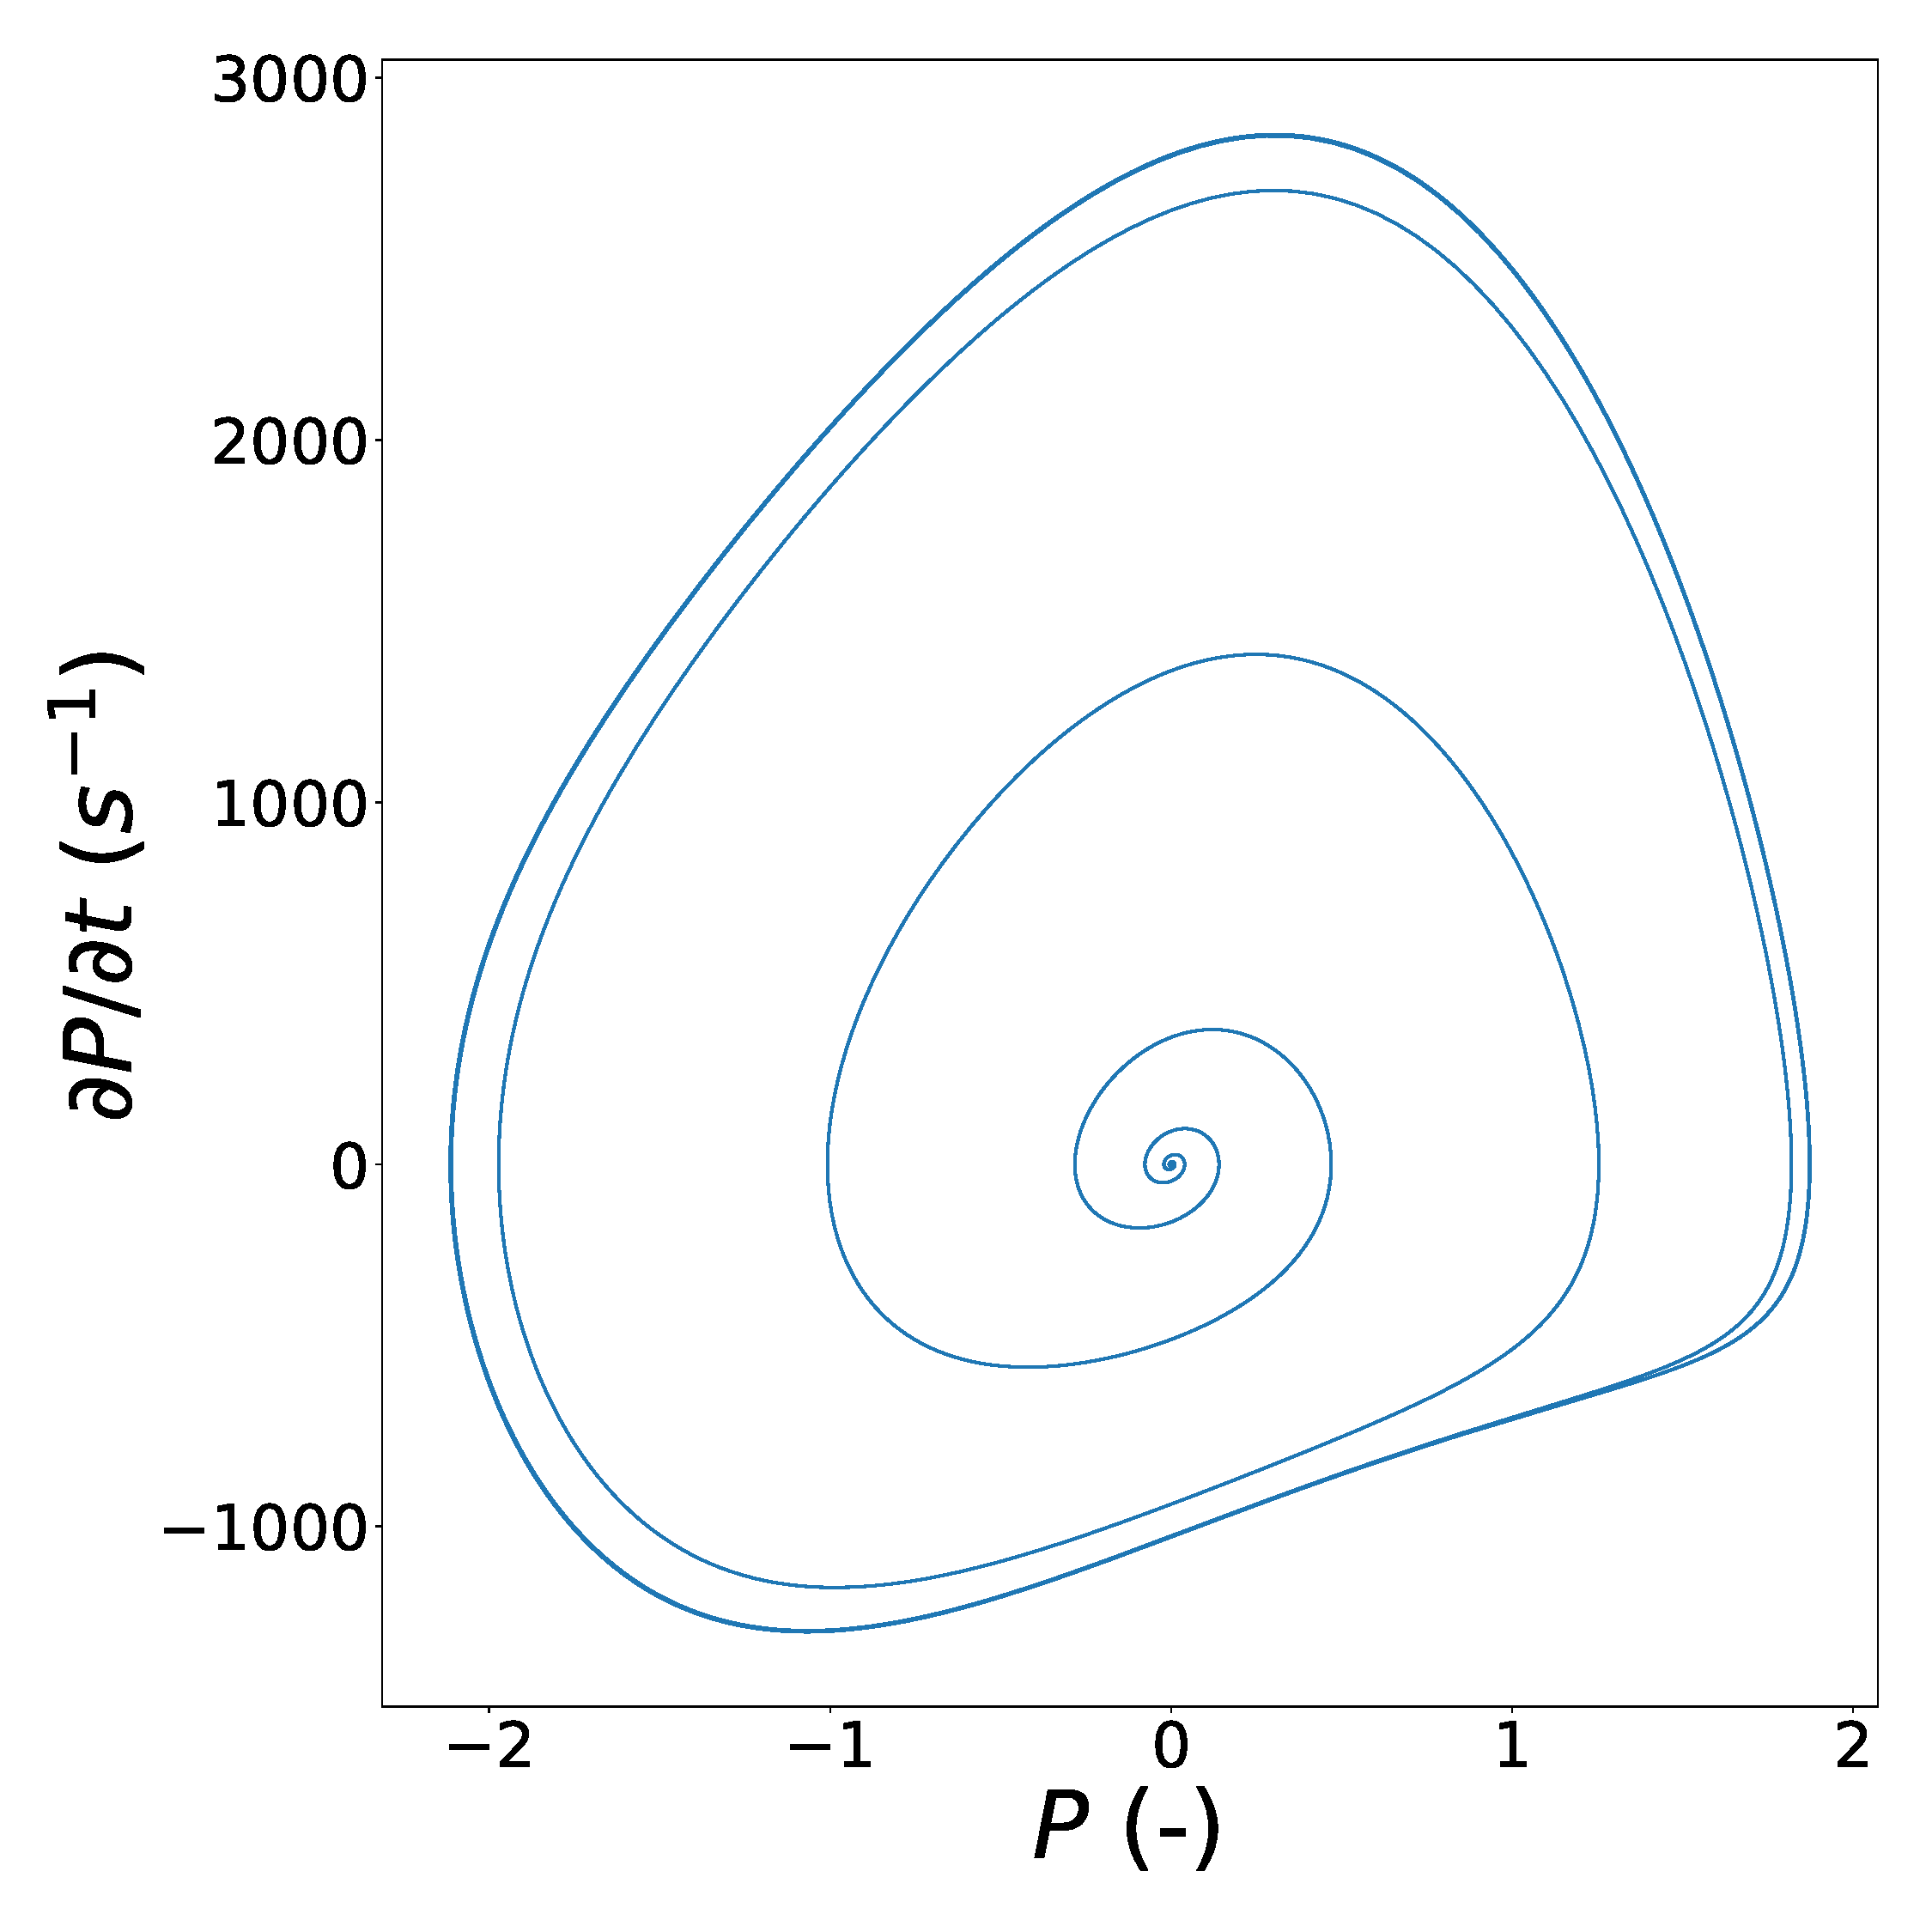
\includegraphics[width=\linewidth]{img/phase_diagram_N1.pdf}
        \caption{$N=1$}
        \label{fig:VDP_phase_N1}
    \end{subfigure}
    \hfill
    \begin{subfigure}[b]{.24\linewidth}
        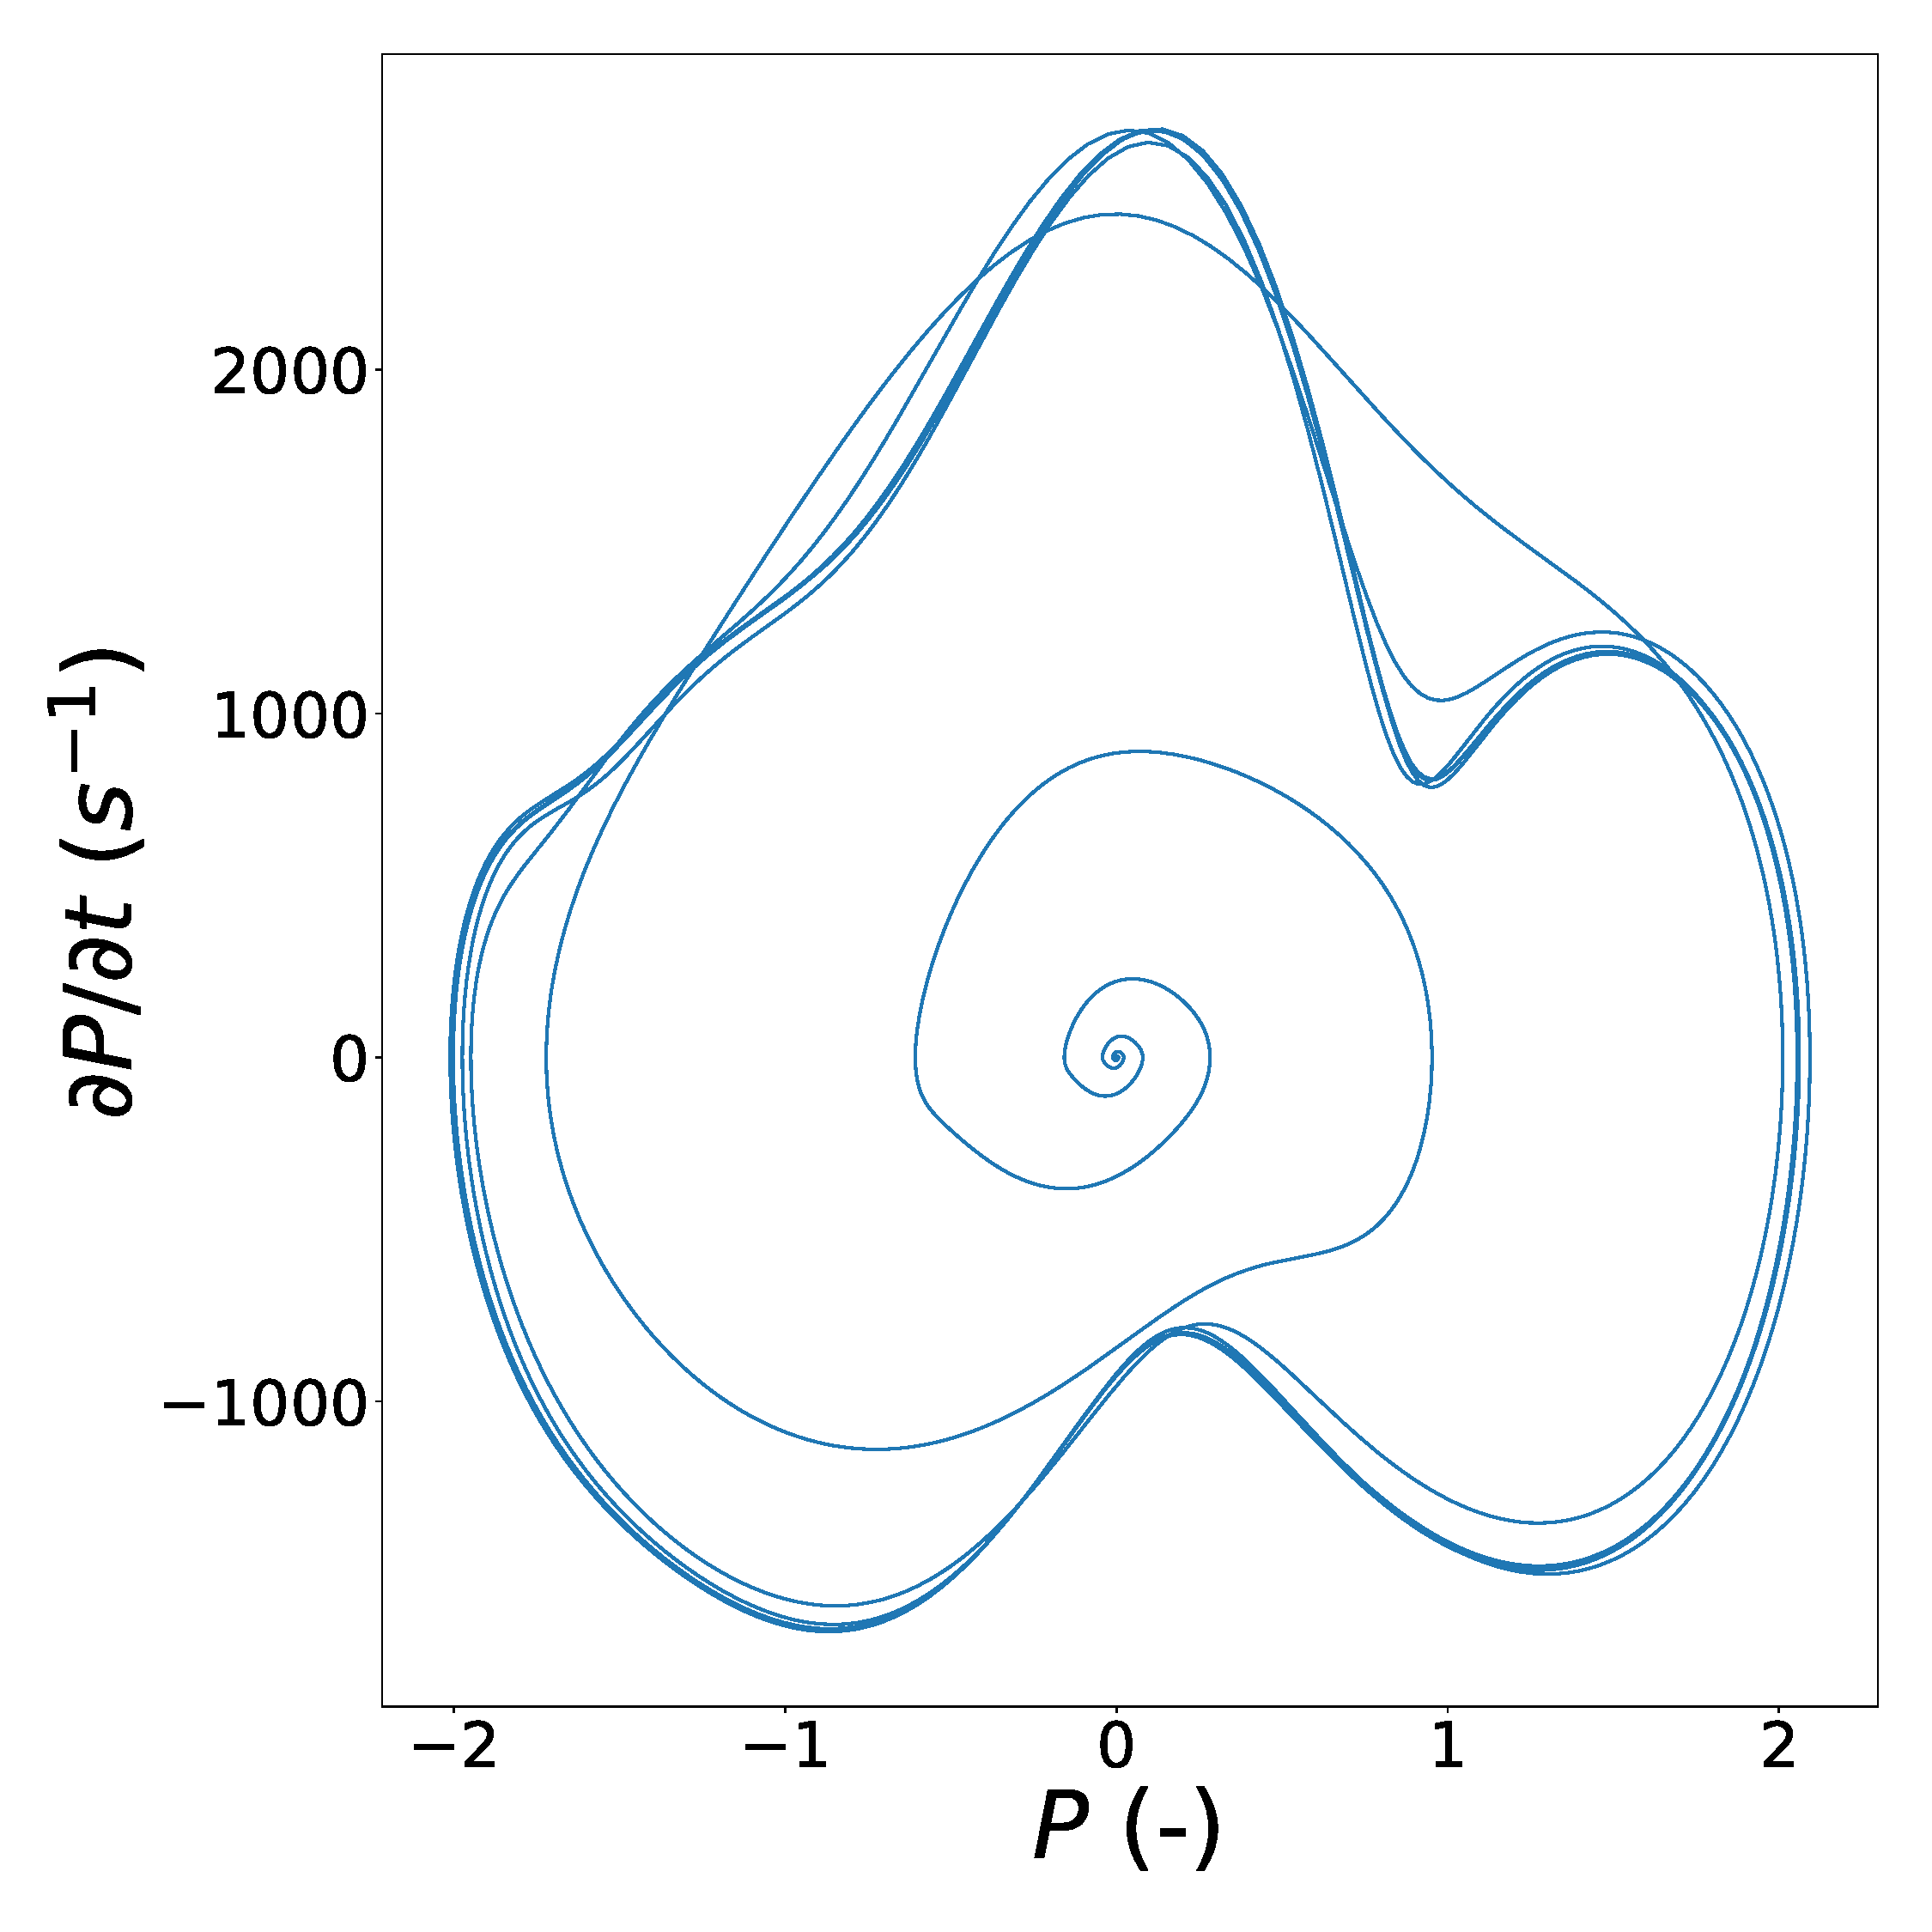
\includegraphics[width=\linewidth]{img/phase_diagram_N2.pdf}
        \caption{$N=2$}
        \label{fig:VDP_phase_N2}
    \end{subfigure}
    \hfill
    \begin{subfigure}[b]{.24\linewidth}
        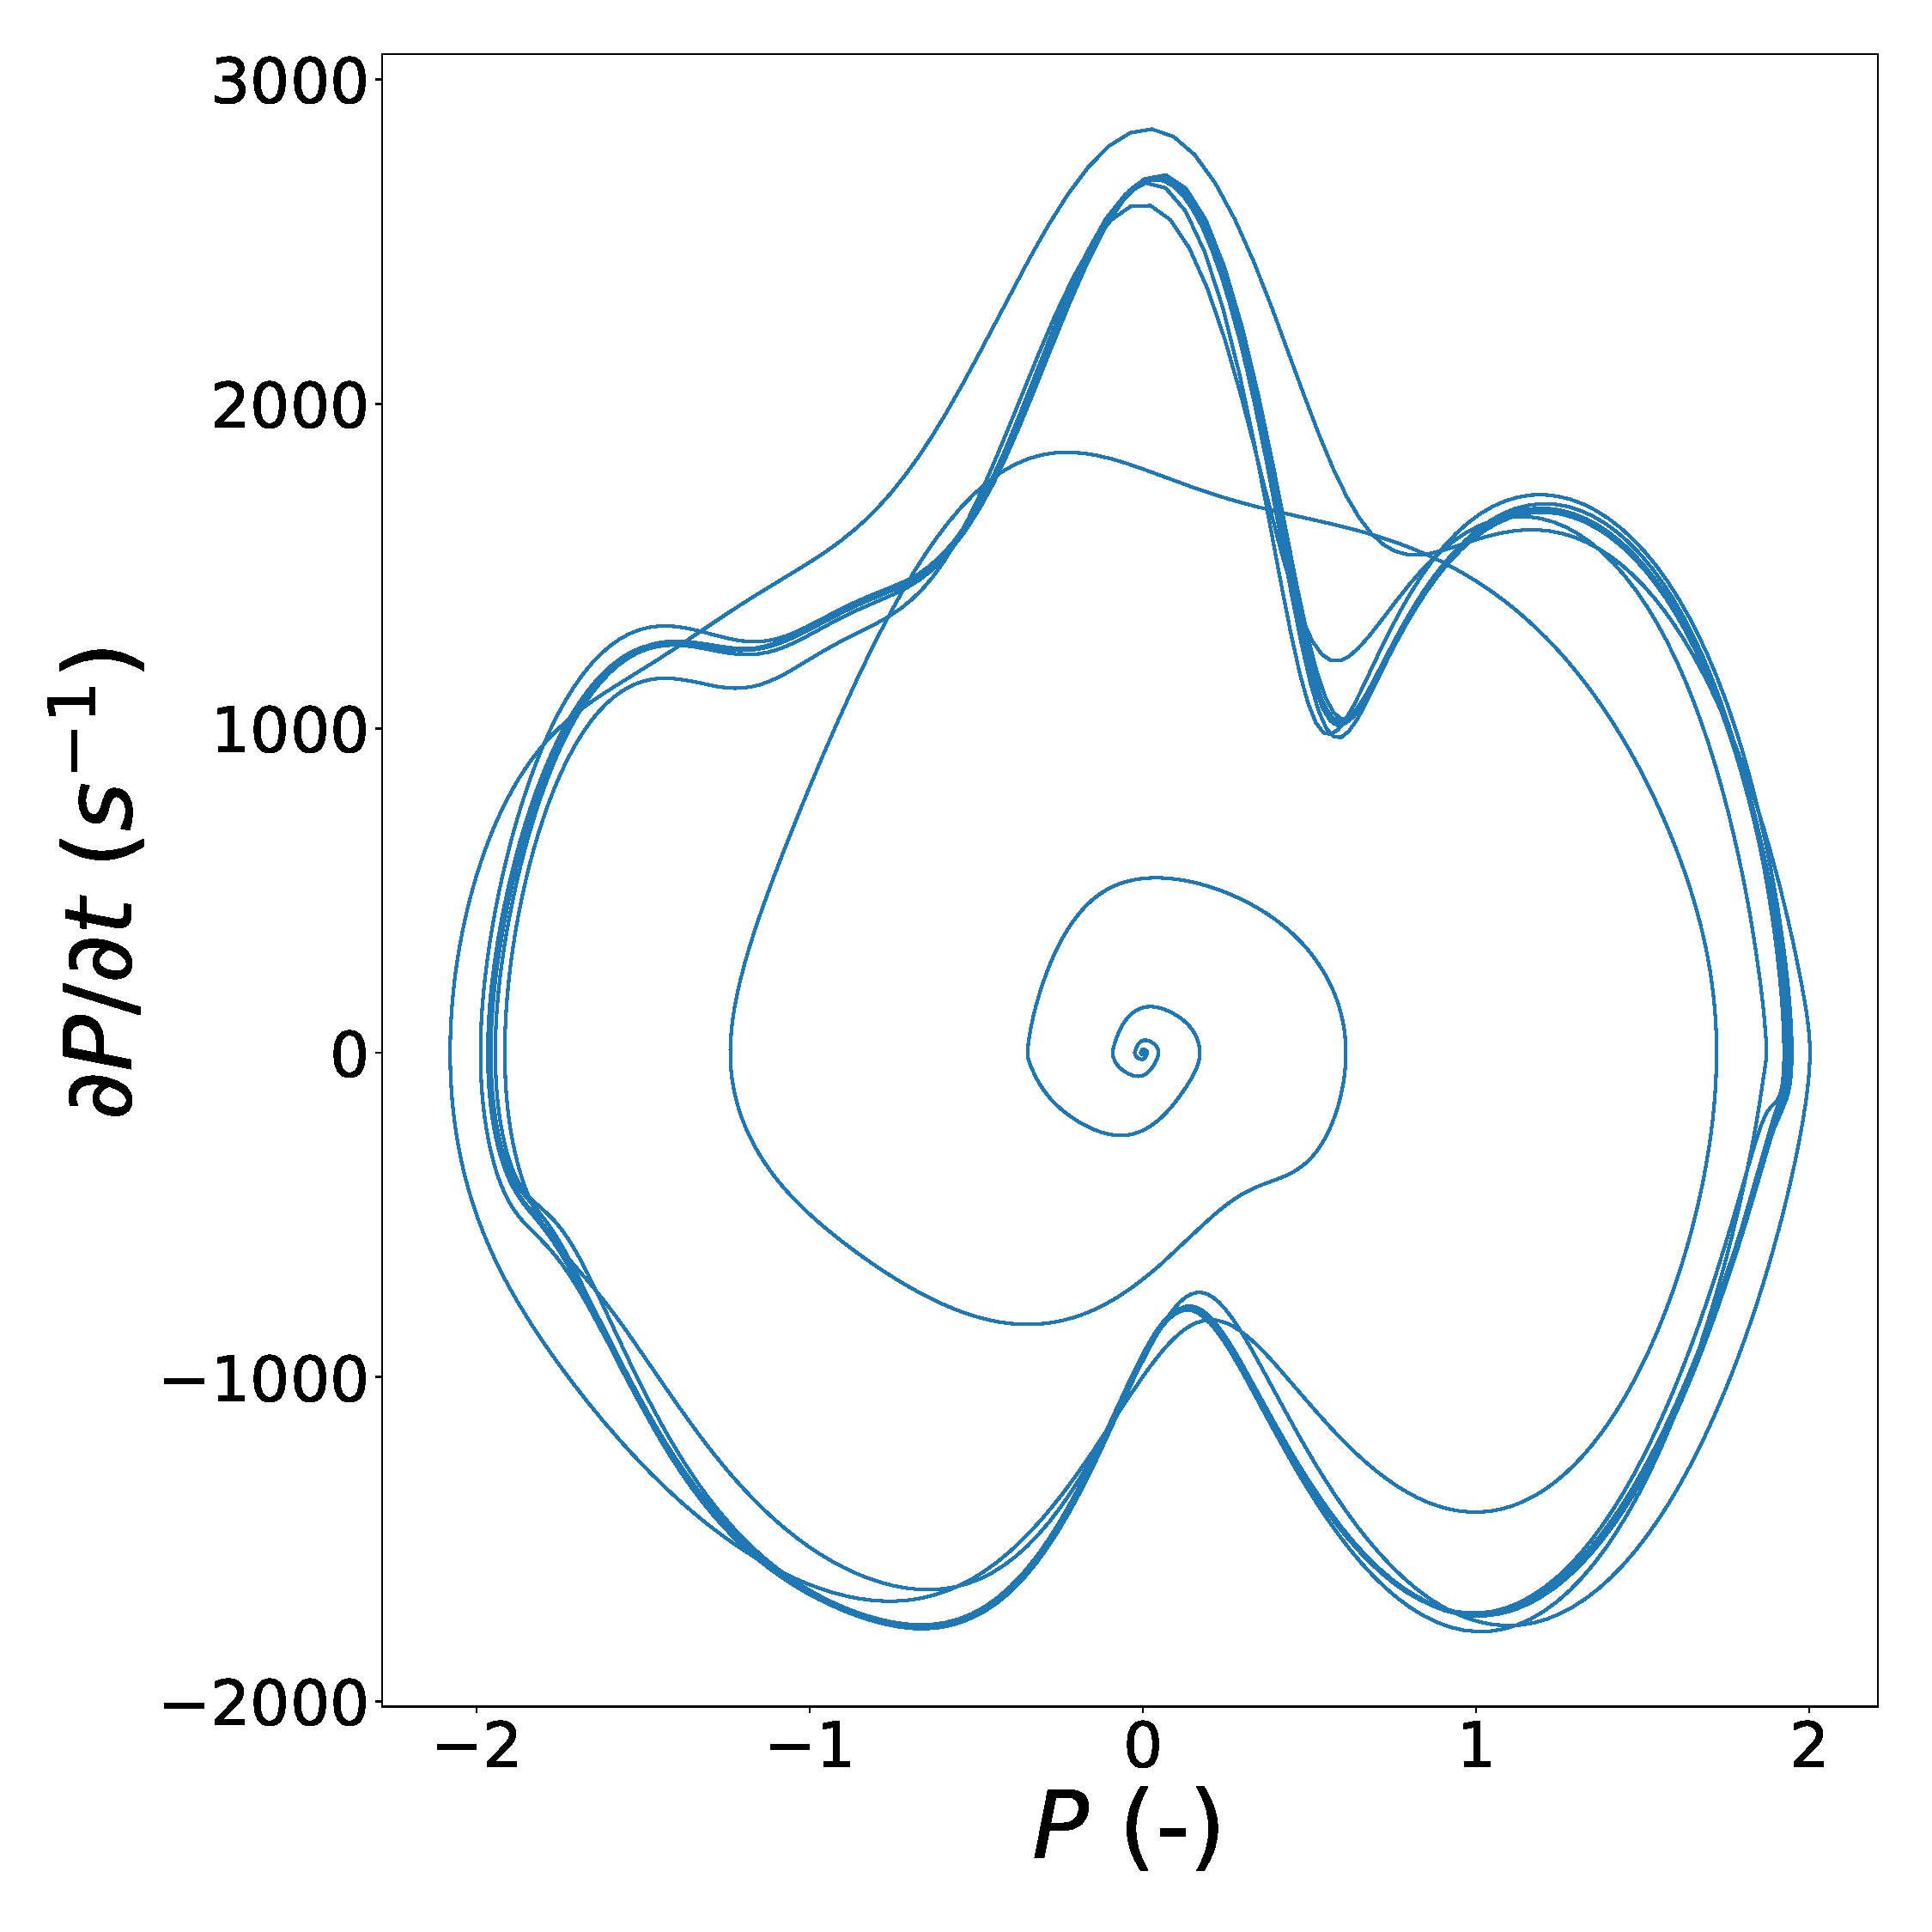
\includegraphics[width=\linewidth]{img/phase_diagram_N3.pdf}
        \caption{$N=3$}
        \label{fig:VDP_phase_N3}
    \end{subfigure}
    \hfill
    \begin{subfigure}[b]{.24\linewidth}
        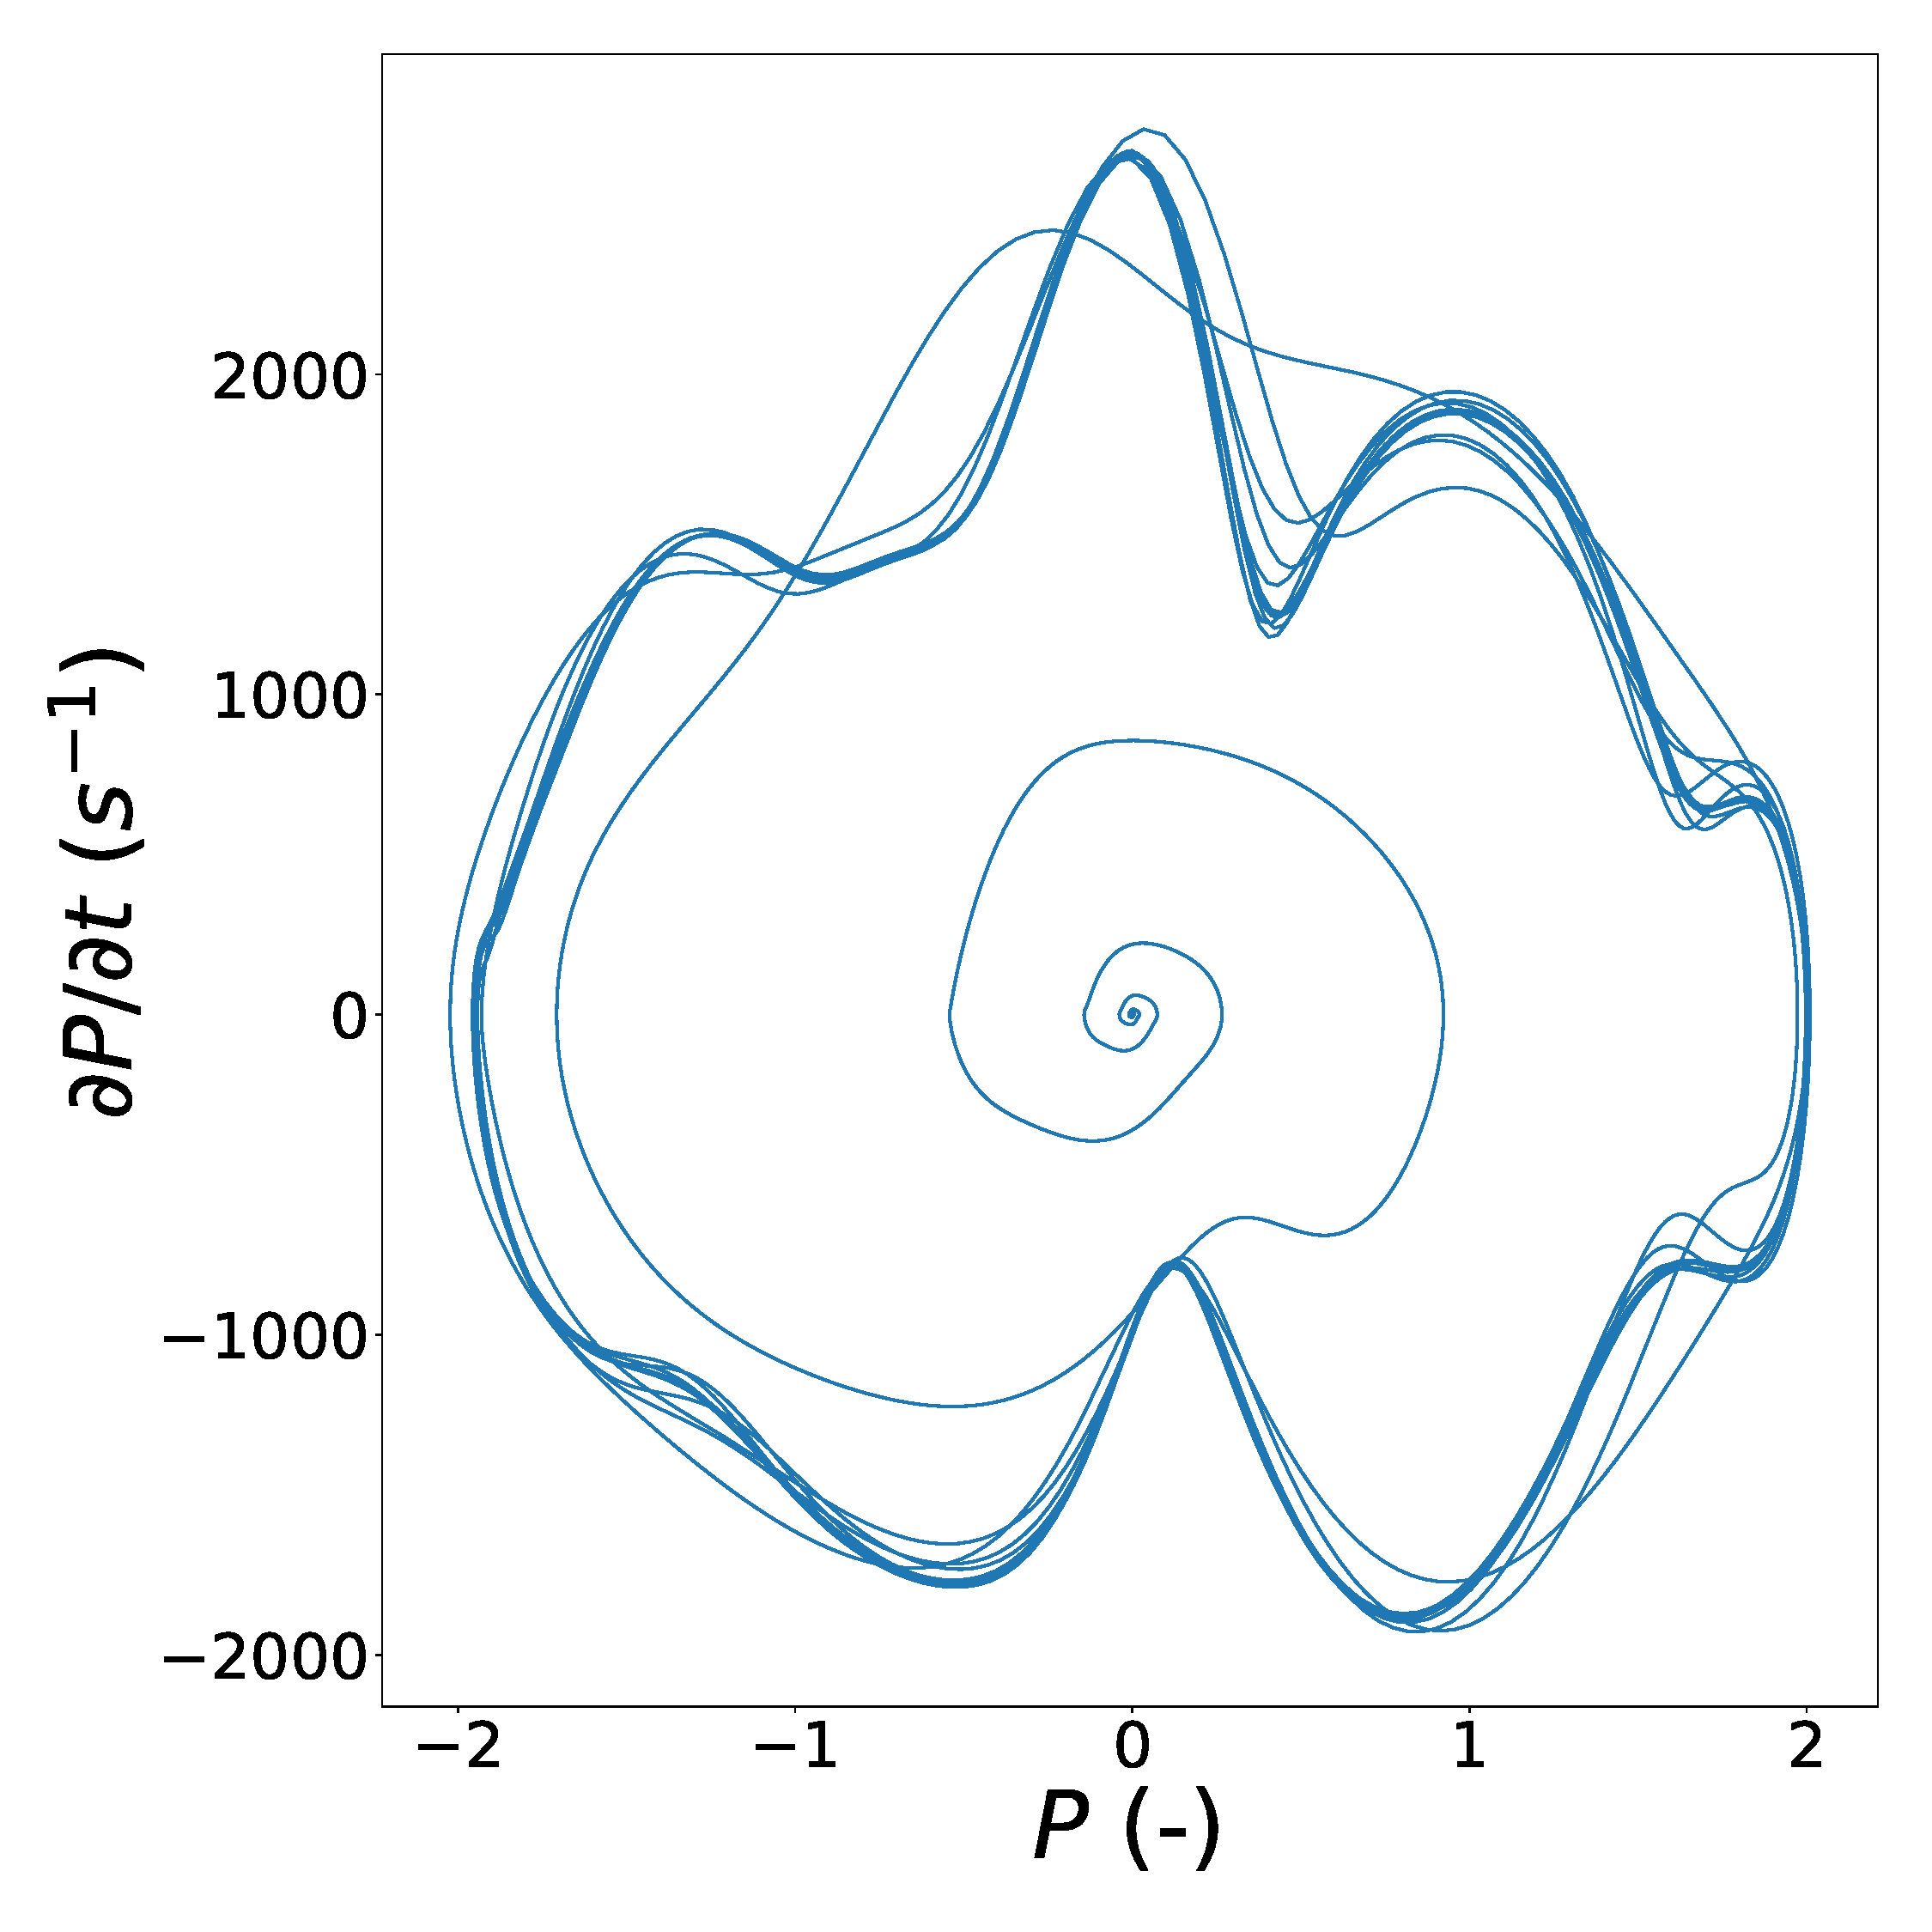
\includegraphics[width=\linewidth]{img/phase_diagram_N4.pdf}
        \caption{$N=4$}
        \label{fig:VDP_phase_N4}
    \end{subfigure}
    \caption{Evolution du flot $(P_0,\frac{\partial P_0}{\partial t})$ dans l'espace des phases durant l'attaque ($t<0.3$ s) pour $N$ modes. Le système est initialement perturbé par un saut de pression $P(t=0)=\epsilon$ ($\epsilon \ll 1$). Les solutions du système d'équations de Van der Pol convergent vers un cycle limite, dont la forme se complexifie avec N.}
    \label{fig:VDP_phase}
\end{figure*}

- résolution numérique : runge kuta

\subsubsection{Cartes itérées}

\subsubsection{Guide d'onde}

Ligne à retard, complexification du modèle pour tenir compte des pertes plus importantes en hautes fréquences.

\section{Implémentation des modèles physiques en temps réel}

\subsection{État de l'art}



% \href{Max MSP}{https://cycling74.com/products/max}




% \subsection{modélisation et résolution}
% - approches analytiques : guide d'onde et modes





\section{Descripteurs}

La clarinette possède des modes de jeu et de régimes sonores divers. Comme pour l'instrument réel, on souhaite étudier et classifier les différents types de jeu disponible grâce à notre instrument numérique. Pour cela, il est nécessaire de définir des descripteurs permettant ensuite de classifier les différents types de jeu en fonction des paramètres d'entrée du modèle $\zeta$ et $\gamma$. 

\subsection{État de l'art}
% \subsubsection{Descripteur/ méthode de classification : cartographie}
\paragraph{Descripteurs : Présence de son}
%Description des bifurcation et donc de l'apparition possible de branches de solutions périodiques par étude de la solution linéarisée \cite{chaigne2008acoustique}. 
On définit la présence de son comme \cite{missoum_explicit_2014}: 

\begin{equation*}
    \frac{1}{N}\sum_{N}p(t_i)>\epsilon  
\end{equation*}

%\begin{equation*}
%    \frac{1}{N}\sum_{N}p(t_i)< \epsilon
%\end{equation*}
Avec $\epsilon$ un seuil choisis.

\paragraph{Descripteur : Justesse}
On peut définir l'intervalle entre deux notes en cent comme : 
\begin{equation*}
    i = 1200 \log_2 \left( \frac{f_1}{f_2}\right)
\end{equation*}
On peut alors un descripteur de justesse qui caractérise si l'écart entre la fréquence jouée par le modèle est proche, selon un intervalle définit, de la fréquence correspondant au premier mode propre du résonateur. 

On choisis $i=5$ comme limite de proximité entre deux fréquences \cite{missoum_explicit_2014}. 

On peut suivre la même approche pour déterminer la présence de second registre en étudiant la proximité de la présence jouée à la fréquence du second mode du résonateur.

\paragraph{Descripteur : son périodique}
Pour étudier la périodicité du signal, on utilise le signal d'enveloppe du signal de pression. Et définir un critère entre régimes périodiques et pseudo-périodiques comme \cite{doc2014minimal}: 
\begin{equation*}
    \epsilon = \frac{Var(pe)}{\langle pe \rangle}
\end{equation*}


\paragraph{Descripteur : rugosité}
On peut caracteriser la rugosité du son produit par la clarinette. 
La rugosité est définie comme : 

\paragraph{Espace de phase}
Gibiat \cite{gibiat_phase_1988} propose d'utiliser la représentation en espace des phases accompagnée d'une analyse de Fourier pour détecter le comportement multiphonique d'une clarinette. Cette représentation est obtenue en traçant l'évolution des degrés de liberté du système ou dans le cas d'une réduction à un degré de liberté principal, la représentation du degré de liberté à un instant $t$ et $t + \tau$. 

En effet, la représentation dans l'espace des phases propose une lecture graphique intéressante des phénonomènes vibratoires de la clarinette. Une première tentative à été d'essayer de construire un descripteur pour identifier le registre utilisé sur des enregistrements réels où cette information nous est connue. 

Malheureusement, même si deux registres se distinguent bien graphiquement, il a été difficile de construire un algorithme simple pour distinguer les registres les uns des autres. Deux tentatives ont été menées : la première, assez bancale, consistait à compter le nombre de points à vitesse lente (en dessous d'un seuil), mais cette méthode était trop sensible à de faibles variations de timbre. La deuxième consistait à colorier une image avec la courbe obtenue en considérant le nombre de pixels coloriés (plus cette valeur est grande, plus la trajectoire est irrégulière). Malheureusement, cette information n'était pas suffisante pour extraire des informations fiables.

\begin{figure}
    \centering
    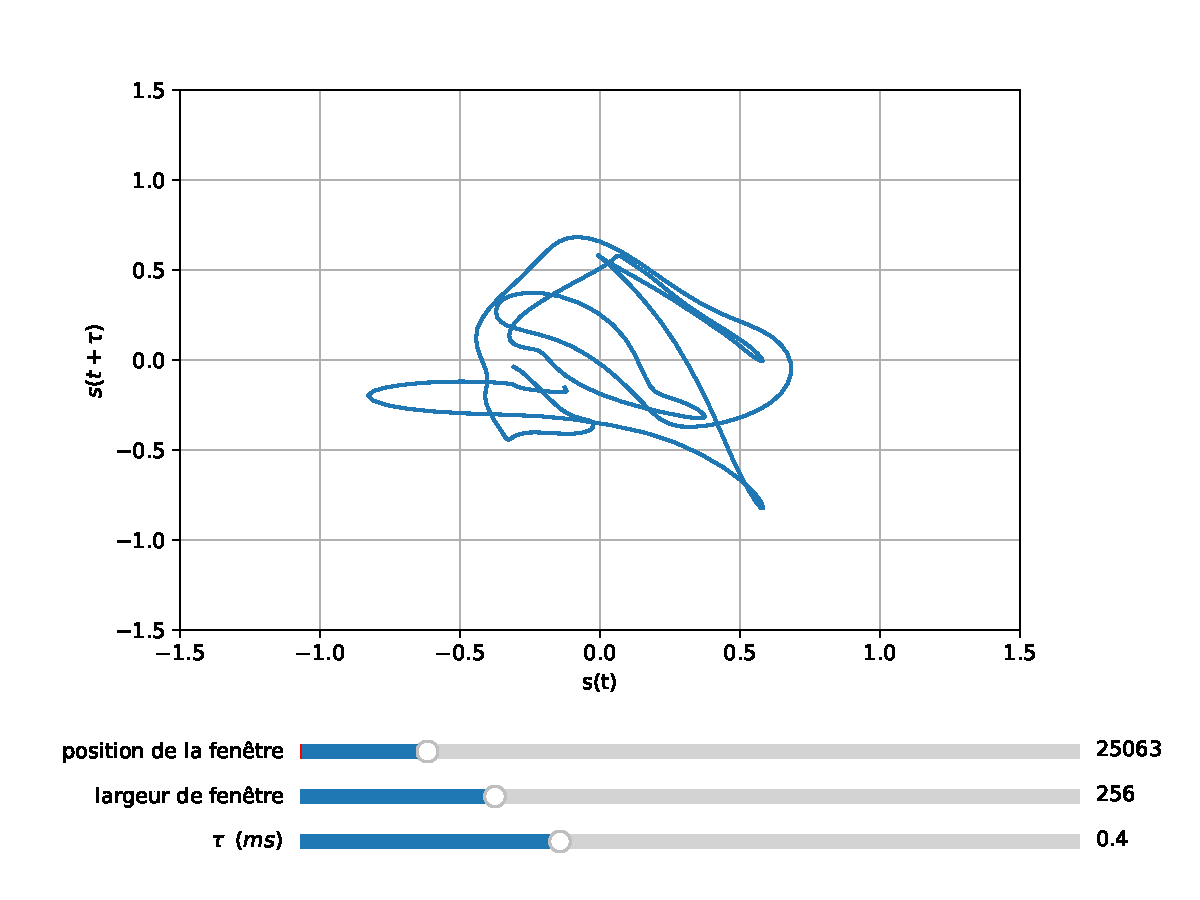
\includegraphics[width=\columnwidth]{Descripteurs/images/espace_des_phases_premier_registre.pdf}
    \caption{Portait de phase de la note Ré (premier registre)}
    \label{phase-reg-1}
\end{figure}

\begin{figure}
    \centering
    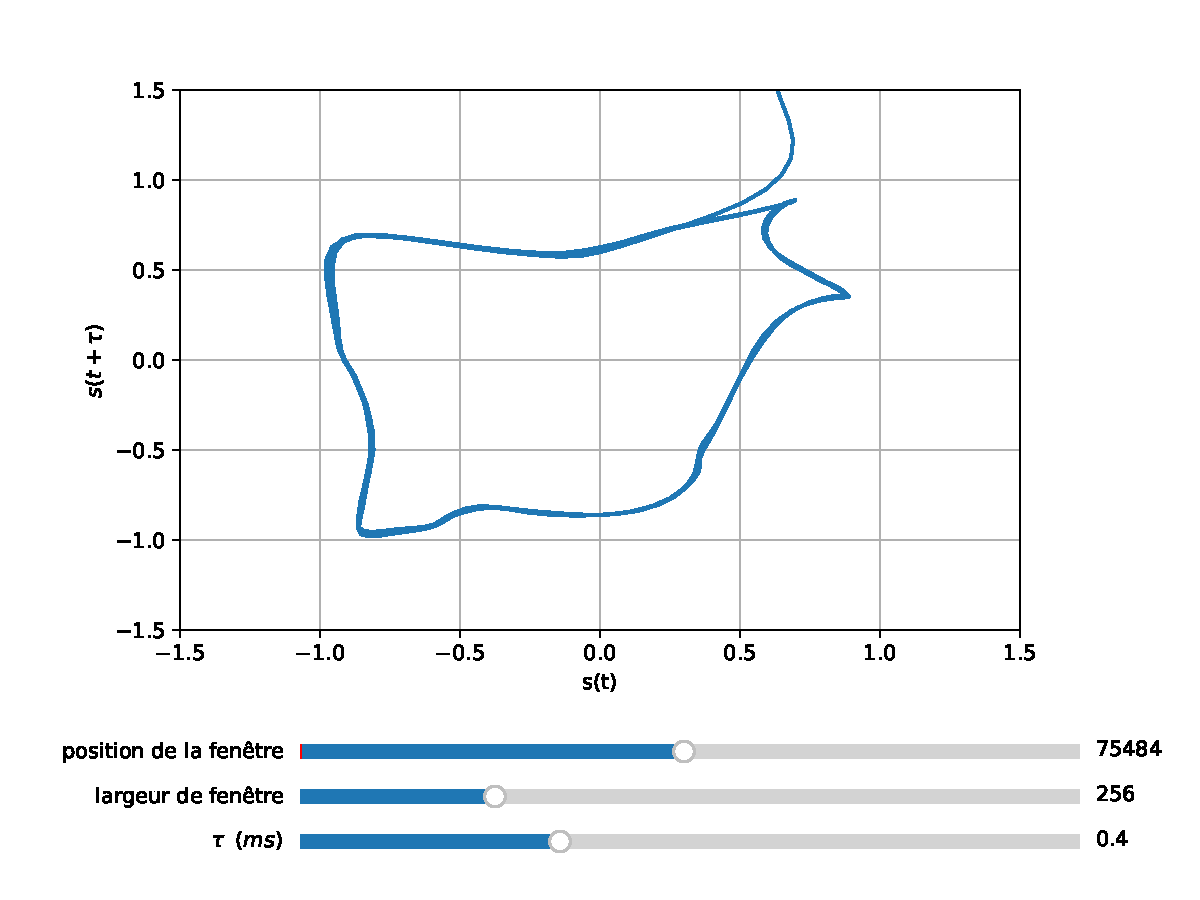
\includegraphics[width=\columnwidth]{Descripteurs/images/espace_des_phases_second_registre.pdf}
    \caption{Portait de phase de la note La (deuxième registre)}
    \label{phase-reg-2}
\end{figure}

\paragraph{SVM}

Bien souvent, les descripteurs sont longs à évaluer pour des raison de temps de calcul. Ainsi, un grand nombre d'évaluations n'est pas possible pour cartographier l'espace des paramètres. Une manière d'interpoler les descripteurs sur l'espace des paramètres échantillonné grossièrement est de d'utiliser une SVM (\textit{state vector machine}). Cette dernière fait apparaître une frontière de décision continue permettant d'interpoler les descripteur sur l'espace des paramètres qui est meilleure que d'utiliser la valeur du voisin le plus proche.

En général, une cartographie peut être réalisée en quadrillant l'espace des paramètres et en évaluant les descripteurs en un point de chaque cellule. Cependant, pour éviter d'avoir recours à un quadrillage trop fin, une méthode d'échantillonnage adaptatif est employée. Cette méthode consiste à évaluer les points de la frontière qui présentent le plus d'incertitude (ceux qui sont loin des points déjà évalués).

\subsection{Méthodes et résultats}



\section{Contrôle}
\subsection{État de l'art}

\subsection{Implémentation et interface temps réel : max}




% \section{Méthodes et résultats}
% \subsection{Méthode}




% \subsubsection{Méthode d'évaluation du dispositif}

\subsubsection{cartographie}
\section{Évaluation du dispositif}
apprécier en situation de jeu/intérêt de l'intérêt : évaluation de l'instrument créé. (réalisme, jouabilité, compréhension de la physique : outil didactique)  %

\section{Conclusion et perspectives}

\begin{comment}
    axe d'approche "type PAM"
        aborder les éléments appris pendant le projet en plus des contributions.
\end{comment}

Perspectives : rappel de l'état de l'art pour adapter notre travail à un instrument à cordes frottées -> perspective logique pour appliquer le travail à d'autres instruments (à voir si on peut utiliser l'approche modale ou si l'analogie est vraie qu'en guide d'ondes).
% \newpage

\fancypagestyle{plain}{plain}
 {\hypersetup{hidelinks} \printbibliography }


\end{document}